\chapter{\IfLanguageName{dutch}{Server installatie en configuratie}{Introduction}}
\label{ch:serverconf}
Dit hoofdstuk voert een tweede onderzoek. Er wordt gekeken hoe makkelijk een volledig type server wordt geïnstalleerd en geïmplementeerd. 

De twee type servers die worden geïnstalleerd zijn: MySQL en LAMP.

\section{LAMP server}
Een LAMP server is een van de populairste variaties van een webserver op linux. Via de documentatie van \autocite{lamp} wordt een kleine uitleg gegeven.

De 'L' staat voor Linux het besturingssysteem dat op de server draait. 

De 'A' staat voor apache dit is de web server software. 

De 'M' kan voor 2 dingen staan: MariaDB of MySQL. Dit zijn de database server softwares die worden gebruikt. In deze setup wordt gekozen voor MariaDB aangezien er al een aparte MySQL server wordt aangemaakt.

De 'P' staat voor PHP. Dit is de programmeer taal die de websites zullen gebruiken.

Een variatie op LAMP is LEMP. Dit is bijna hetzelfde alleen gebruikt het nginx als web server software in plaats van apache.


\subsection{Cloud-init}
Het bestand werd opgemaakt met behulp van \autocite{butcher}. Hierdoor krijgen we een basis lamp stack.

Allereerst werd het cloud-init script opgemaakt. Het script bevat niet zoveel functies. Het bevat 3 modules: \textit{package\_upgrade}(voor het updaten van de server packages), \textit{packages} (voor de packages die nodig zijn) en \textit{runcmd} (voor de taken die moeten worden uitgevoerd).

\subsubsection{Opmaken bestand}
\textit{Package\_upgrade} wordt allereerst op true gezet. Bij de \textit{packages} wordt: \textit{apache2, mysql-server, libapache2-mod-php5} en \textit{php5-mysql} gezet. Dit zijn de packages dit nodig zijn voor de lamp stack.
\begin{lstlisting}[basicstyle=\small]
package_upgrade: true

packages:
- apache2
- mysql-server
- libapache2-mod-php5
- php5-mysql
\end{lstlisting}

Bij \textit{runcmd} werden 2 commando's geplaats. Het eerste maakt het php bestand aan dat de server gaat gebruiken. Het tweede verwijdert het standaard html bestand.
\begin{lstlisting}[basicstyle=\small]
runcmd:
- echo '<?php phpinfo();' > /var/www/html/index.php
- rm /var/www/html/index.html
\end{lstlisting}


\subsection{Ansible}
Dit bestand werd opgemaakt met behulp van \autocite{bekker}. Dit maakt een basis lamp stack aan. Het playbook is onderverdeeld in 3 delen: installeren van de packages, starten van de services en het  toevoegen van het php bestand.

\subsubsection{Installeren packages}
Eerst en vooral worden de packages geïnstalleerd: \textit{apache2, my-sqlserver, php} en \textit{php-mysql}.
\begin{lstlisting}[basicstyle=\small]
- name: install lamp stack
become: yes
become_user: root
apt:
pkg:
- apache2
- mysql-server
- php
- php-mysql
state: present
update_cache: yes
\end{lstlisting}

\subsubsection{Starten services}
Als tweede werden de \textit{apache2} en \textit{mysql} server gestart. 
\begin{lstlisting}[basicstyle=\small]
- name: start apache service
become: yes
become_user: root
service:
name: apache2
state: started
enabled: yes

- name: start mysql service
become: yes
become_user: root
service:
name: mysql
state: started
enabled: yes
\end{lstlisting}

\subsubsection{Php bestand}
Ten laatste werd het php bestand aangemaakt en de map waar het moet komen. Het bestand kon via Ansible wel niet worden aangemaakt. Dus werd het via github meegeven. Het stond ook in de repo van het playbook.
\begin{lstlisting}[basicstyle=\small]
- name: create target directory
file: path=/var/www/html state=directory mode=0755

- name: deploy index.php
become: yes
become_user: root
copy:
src: /repo/index.hphp
dest: /var/www/html/index.php
\end{lstlisting}

\subsection{Cloud-init \& Ansible}
\label{ch:cloudansiserverconf}
Voor de configuratie van Ansible en cloud-init worden de taken in 2 verdeeld. 

De packages worden geinstalleerd via cloud-init. Ook het aanmaken van het php bestand gebeurt via cloud-init. Het starten van de services wordt gedaan door Ansible ook het aanmaken van de directory wordt gedaan door Ansible.

\section{MySQL server}
De tweede server die werd gekozen is een MySQL server. MySQL is een database management systeem (DBMS). Een MySQL server is dus simpel weg een database server.

\subsection{Cloud-init}
Dit bestand werd opgemakt met behulp van \autocite{dias}.

Voorr het aanmaken van een MySQL server werden 3(4) modules gebruikt. Allereest de \textit{packages} (en \textit{package\_upgrade}) voor de packages, \textit{users} voor de database user en \textit{runcmd} voor de taken/commando's.

\subsubsection{Packages}
De packages die werden geïnstalleerd zijn: \textit{mysql-client, libmysqclient-dev} en \textit{mysql-server}.
\begin{lstlisting}[basicstyle=\small]
packages:
- mysql-client
- libmysqlclient-dev
- mysql-server

package_upgrade: true
\end{lstlisting}

\subsubsection{User}
Er werd een gebruiker toegevoegd dev. Met een ssh sleutel zodat er toegang is via deze gebruiker.
\begin{lstlisting}[basicstyle=\small]
users:
- name: dev
ssh-authorized-keys:
- ssh-rsa <key>
sudo: ['ALL=(ALL) NOPASSWD:ALL']
groups: sudo
shell: /bin/bash
\end{lstlisting}

\subsubsection{Commando's}
Ten laatste al de commando's die worden uitgevoerd. Hier wordt de mysql server geconfigureerd.
\begin{lstlisting}[basicstyle=\small]
runcmd:
- sed -i -e '/^Port/s/^.*$/Port 22/' /etc/ssh/sshd_config
- sed -i -e '/^PermitRootLogin/s/^.*$/PermitRootLogin no/' /etc/ssh/sshd_config
- sed -i -e '/^PasswordAuthentication/s/^.*$/PasswordAuthentication no/' /etc/ssh/sshd_config
- sed -i -e '$aAllowUsers dev' /etc/ssh/sshd_config
- sudo service ssh restart
- sudo ufw default deny incoming
- sudo ufw default allow outgoing
- sudo ufw allow ssh
- sudo ufw allow http
- sudo ufw allow https
- sed -i -e '/^ENABLED/s/^.*$/ENABLED=yes/' /etc/ufw/ufw.conf
- sudo ufw enable
\end{lstlisting}


\subsection{Ansible}
Dit bestand werd gemaakt met behulp van \autocite{hassin}.

Allereest werden weer de my-sql packages geïnstalleerd.
\begin{lstlisting}[basicstyle=\small]
- name: install my-sql
become: yes
become_user: root
apt:
pkg:
- mysql-server-core-5.7
- mysql-client-core-5.7
- libmysqlclient-dev
- python-mysqldb
- mysql-server
- mysql-client
\end{lstlisting}

Hierna werden de my-sql configuraties gedaan: het starten van de service, verwijderen van de test database, een my-sql gebruiker aanmaken, anonieme gebruikers verwijderen en het wachtwoord aanpassen voor de root gebruiker.
\begin{lstlisting}[basicstyle=\small]
- name: Start the MySQL service
action: service name=mysql state=started

- name: Remove the test database
mysql_db: name=test state=absent

- name: Create deploy user for mysql
mysql_user: user="deploy" host="%" password=maarten priv=*.*:ALL,GRANT

- name: Ensure anonymous users are not in the database
mysql_user: user='' host=localhost state=absent
with_items:
- 127.0.0.1
- ::1
- localhost

- name: Update mysql root password for all root accounts
mysql_user: name=root host=localhost password=maarten
with_items:
- 127.0.0.1
- ::1
- localhost
\end{lstlisting}


\subsection{Cloud-init \& Ansible}
Voor de configuratie van cloud-init en Ansible werden gelijkaardige dingen gedaan als bij LAMP. In principe werden bijna alle configuraties weer gedaan door Ansible. Alleen werden de packages geïnstalleerd door cloud-init.

\section{Uitvoering \& resultaten}
\subsection{Complexiteit}
Allereerst wordt de complexiteit weer bekeken. Daarin is er een verschil tussen MySQL en LAMP.

Bij de LAMP server is door de weinige configuraties, het cloud-init bestand heel overzichtelijk. Maar bij de MySQL server is dit dan weer niet. Doordat er verschillende configuraties worden gedaan en deze allemaal in de \textit{runcmd} module worden gedaan, is het bestand niet zo duidelijk. 

Bij Ansible daarentegen zijn er door de verschillende modules allemaal verschillende taken hiervoor apart. In deze setup zijn die verschillende taken wel overzichtelijk. 

Ook kunnen er met Ansible meer geavanceerde configuraties worden uitgevoerd bij beide servers. Cloud-init is beperkt tot de configuraties die via een commando kunnen worden gedaan. Ansible kan veel meer uitvoeren. 


\subsection{Snelheid}
Qua snelheden is het vrij duidelijk. Ansible is veel efficiënter en sneller in het uitvoeren van de taken dan ``Ansible en cloud-init'' en cloud-init. Het verschil zonder de initiële configuraties doet er zelf niet toe. 

Dit is, t.o.v het vorige hoofdstuk, wel een verschil dat merkbaar is. Waardoor Ansible in dit onderdeel duidelijk de beter is ten opzichte van de andere 2 opties.

Ook is t.o.v. het vorige hoofdstuk het verschil tussen cloud-init en ``Ansible en cloud-init'' veel groter.

\begin{table}[!htb]
    \centering
    \begin{tabular}{| l | l | l |l |}
        \hline
        \textbf{Uitvoeringstijd} & Resultaat 1 & Resultaat 2 & Resultaat 3   \\ \hline
        cloud-init & 230.57 sec & 229.85 sec & 234.71 sec  \\ \hline
        Anisble & 62.71 sec & 76.10 sec & 65.48 sec \\ \hline
        cloud-init \& Ansible & 150.97 sec & 127.93 sec & 129.80 sec \\
        \hline
    \end{tabular}
    \caption{Snelheid tabel van LAMP configuraties op de servers.}
    \label{tab:tabel lamp resultaten server}
\end{table}

\begin{table}[!htb]
    \centering
    \begin{tabular}{| l | l | l |l |}
        \hline
        \textbf{Uitvoeringstijd} & Resultaat 1 & Resultaat 2 & Resultaat 3   \\ \hline
        cloud-init & 204.03 sec & 214.15 sec & 281.82 sec  \\ \hline
        Anisble & 29.26 sec & 35.86 sec & 111.31 sec \\ \hline
        cloud-init \& Ansible & 127.71 sec & 85.43 sec & 66.81 sec \\
        \hline
    \end{tabular}
    \caption{Snelheid tabel van MySQL configuraties op de servers.}
    \label{tab:tabel mysql resultaten server}
\end{table}

\subsection{Resultaat}
Voor server configuratie is het duidelijk dat Ansible de beste optie is. Ansible is veel sneller, overzichtelijker en heeft veel meer opties om te configureren. 

Ook door de output die Ansible geeft (Figuur \ref{fig:Ansibleoutput}) is het veel makkelijker om fouten uit een server configuratie te halen. Door de vele configuratie die deze scripts soms hebben, is het overzichtelijk dat in de output alles is opgelijst als 1 taak.
\begin{figure}[!htb]
    \center{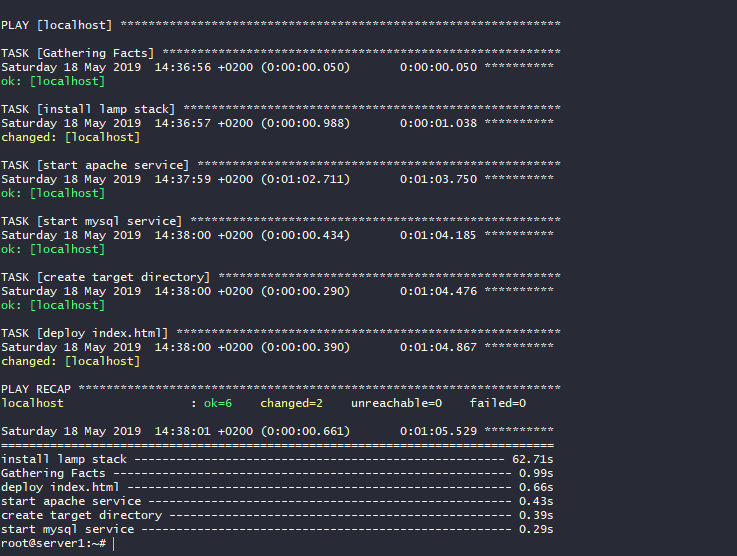
\includegraphics[width=0.9\textwidth]{img/ansibleoutput.png}}
    \caption{Ansible output voorbeeld.}
    \label{fig:Ansibleoutput}
\end{figure}

Al is cloud-init niet helemaal nutteloos hier. Als er bij de opstart van de server deze configuraties moeten worden gedaan. Is het de beste optie om cloud-init en Ansible te gebruiken. Doordat het cloud-init veel makkelijker kan worden meegegeven als een variabele. In dit script wordt er dan verwezen naar het Ansible playbook.
